\documentclass[manuscript, review, anonymous, screen]{acmart}


\IfFileExists{upquote.sty}{\usepackage{upquote}}{}
\IfFileExists{microtype.sty}{% use microtype if available
  \usepackage[]{microtype}
  \UseMicrotypeSet[protrusion]{basicmath} % disable protrusion for tt fonts
}{}
\makeatletter
\@ifundefined{KOMAClassName}{% if non-KOMA class
  \IfFileExists{parskip.sty}{%
    \usepackage{parskip}
  }{% else
    \setlength{\parindent}{0pt}
    \setlength{\parskip}{6pt plus 2pt minus 1pt}}
}{% if KOMA class
  \KOMAoptions{parskip=half}}
\makeatother

%%
%% This is file `sample-manuscript.tex',
%% generated with the docstrip utility.
%%
%% The original source files were:
%%
%% samples.dtx  (with options: `manuscript')
%% 
%% IMPORTANT NOTICE:
%% 
%% For the copyright see the source file.
%% 
%% Any modified versions of this file must be renamed
%% with new filenames distinct from sample-manuscript.tex.
%% 
%% For distribution of the original source see the terms
%% for copying and modification in the file samples.dtx.
%% 
%% This generated file may be distributed as long as the
%% original source files, as listed above, are part of the
%% same distribution. (The sources need not necessarily be
%% in the same archive or directory.)
%%
%%
%% Commands for TeXCount
%TC:macro \cite [option:text,text]
%TC:macro \citep [option:text,text]
%TC:macro \citet [option:text,text]
%TC:envir table 0 1
%TC:envir table* 0 1
%TC:envir tabular [ignore] word
%TC:envir displaymath 0 word
%TC:envir math 0 word
%TC:envir comment 0 0
%%
%%
%% The first command in your LaTeX source must be the \documentclass command.


% Options for packages loaded elsewhere
\PassOptionsToPackage{unicode}{hyperref}
\PassOptionsToPackage{hyphens}{url}
\PassOptionsToPackage{dvipsnames,svgnames,x11names}{xcolor}

\IfFileExists{bookmark.sty}{\usepackage{bookmark}}{\usepackage{hyperref}}

%% PANDOC PREAMBLE BEGINS


\providecommand{\tightlist}{%
  \setlength{\itemsep}{0pt}\setlength{\parskip}{0pt}}\usepackage{longtable,booktabs,array}
\usepackage{calc} % for calculating minipage widths
% Correct order of tables after \paragraph or \subparagraph
\usepackage{etoolbox}
\makeatletter
\patchcmd\longtable{\par}{\if@noskipsec\mbox{}\fi\par}{}{}
\makeatother
% Allow footnotes in longtable head/foot
\IfFileExists{footnotehyper.sty}{\usepackage{footnotehyper}}{\usepackage{footnote}}
\makesavenoteenv{longtable}
\usepackage{graphicx}
\makeatletter
\def\maxwidth{\ifdim\Gin@nat@width>\linewidth\linewidth\else\Gin@nat@width\fi}
\def\maxheight{\ifdim\Gin@nat@height>\textheight\textheight\else\Gin@nat@height\fi}
\makeatother
% Scale images if necessary, so that they will not overflow the page
% margins by default, and it is still possible to overwrite the defaults
% using explicit options in \includegraphics[width, height, ...]{}
\setkeys{Gin}{width=\maxwidth,height=\maxheight,keepaspectratio}
% Set default figure placement to htbp
\makeatletter
\def\fps@figure{htbp}
\makeatother

\usepackage{booktabs}
\usepackage{longtable}
\usepackage{array}
\usepackage{multirow}
\usepackage{wrapfig}
\usepackage{float}
\usepackage{colortbl}
\usepackage{pdflscape}
\usepackage{tabu}
\usepackage{threeparttable}
\usepackage{threeparttablex}
\usepackage[normalem]{ulem}
\usepackage{makecell}
\usepackage{xcolor}
\definecolor{mypink}{RGB}{219, 48, 122}
\makeatletter
\makeatother
\makeatletter
\makeatother
\makeatletter
\@ifpackageloaded{caption}{}{\usepackage{caption}}
\AtBeginDocument{%
\ifdefined\contentsname
  \renewcommand*\contentsname{Table of contents}
\else
  \newcommand\contentsname{Table of contents}
\fi
\ifdefined\listfigurename
  \renewcommand*\listfigurename{List of Figures}
\else
  \newcommand\listfigurename{List of Figures}
\fi
\ifdefined\listtablename
  \renewcommand*\listtablename{List of Tables}
\else
  \newcommand\listtablename{List of Tables}
\fi
\ifdefined\figurename
  \renewcommand*\figurename{Figure}
\else
  \newcommand\figurename{Figure}
\fi
\ifdefined\tablename
  \renewcommand*\tablename{Table}
\else
  \newcommand\tablename{Table}
\fi
}
\@ifpackageloaded{float}{}{\usepackage{float}}
\floatstyle{ruled}
\@ifundefined{c@chapter}{\newfloat{codelisting}{h}{lop}}{\newfloat{codelisting}{h}{lop}[chapter]}
\floatname{codelisting}{Listing}
\newcommand*\listoflistings{\listof{codelisting}{List of Listings}}
\makeatother
\makeatletter
\@ifpackageloaded{caption}{}{\usepackage{caption}}
\@ifpackageloaded{subcaption}{}{\usepackage{subcaption}}
\makeatother
\makeatletter
\@ifpackageloaded{tcolorbox}{}{\usepackage[skins,breakable]{tcolorbox}}
\makeatother
\makeatletter
\@ifundefined{shadecolor}{\definecolor{shadecolor}{rgb}{.97, .97, .97}}
\makeatother
\makeatletter
\makeatother
\makeatletter
\makeatother
%% PANDOC PREAMBLE ENDS

\setlength{\parindent}{10pt}
\setlength{\parskip}{0pt}

\hypersetup{
  pdftitle={Novel Effects of Size and Contrast Adjustments in Scatterplots},
  pdfauthor={Gabriel Strain; Andrew J. Stewart; Paul Warren; Caroline Jay},
  colorlinks=true,
  linkcolor={blue},
  filecolor={Maroon},
  citecolor={Blue},
  urlcolor={red},
  pdfcreator={LaTeX via pandoc, via quarto}}

%% \BibTeX command to typeset BibTeX logo in the docs
\AtBeginDocument{%
  \providecommand\BibTeX{{%
    Bib\TeX}}}

%% Rights management information.  This information is sent to you
%% when you complete the rights form.  These commands have SAMPLE
%% values in them; it is your responsibility as an author to replace
%% the commands and values with those provided to you when you
%% complete the rights form.
\setcopyright{acmcopyright}
\copyrightyear{2024}
\acmYear{2024}
\acmDOI{XXXXXXX.XXXXXXX}

%% These commands are for a PROCEEDINGS abstract or paper.
\acmConference[CHI]{Make sure to enter the correct conference title from
your rights confirmation email}{June 03--05, 2018}{Honolulu, HI}
\acmPrice{15.00}
\acmISBN{978-1-4503-XXXX-X/18/06}

%% Submission ID.
%% Use this when submitting an article to a sponsored event. You'll
%% receive a unique submission ID from the organizers
%% of the event, and this ID should be used as the parameter to this command.
%%\acmSubmissionID{123-A56-BU3}

%%
%% For managing citations, it is recommended to use bibliography
%% files in BibTeX format.
%%
%% You can then either use BibTeX with the ACM-Reference-Format style,
%% or BibLaTeX with the acmnumeric or acmauthoryear sytles, that include
%% support for advanced citation of software artefact from the
%% biblatex-software package, also separately available on CTAN.
%%
%% Look at the sample-*-biblatex.tex files for templates showcasing
%% the biblatex styles.
%%

%%
%% The majority of ACM publications use numbered citations and
%% references.  The command \citestyle{authoryear} switches to the
%% "author year" style.
%%
%% If you are preparing content for an event
%% sponsored by ACM SIGGRAPH, you must use the "author year" style of
%% citations and references.
%% Uncommenting
%% the next command will enable that style.
%%\citestyle{acmauthoryear}


%% end of the preamble, start of the body of the document source.
\begin{document}


%%
%% The "title" command has an optional parameter,
%% allowing the author to define a "short title" to be used in page headers.
\title[Size, Contrast, and Scatterplots]{Novel Effects of Size and
Contrast Adjustments in Scatterplots}

%%
%% The "author" command and its associated commands are used to define
%% the authors and their affiliations.
%% Of note is the shared affiliation of the first two authors, and the
%% "authornote" and "authornotemark" commands
%% used to denote shared contribution to the research.


  \author{Gabriel Strain}
  \orcid{0000-0002-4769-9221}
            \affiliation{%
                  \institution{Department of Computer Science, Faculty
of Science and Engineering, University of Manchester}
                          \streetaddress{Oxford Road}
                          \city{Manchester}
                                  \country{United Kingdom}
                          \postcode{M13 9PL}
              }
        \author{Andrew J. Stewart}
  
            \affiliation{%
                  \institution{Department of Computer Science, Faculty
of Science and Engineering, University of Manchester}
                          \streetaddress{Oxford Road}
                          \city{Manchester}
                                  \country{United Kingdom}
                          \postcode{M13 9PL}
              }
        \author{Paul Warren}
  
            \affiliation{%
                  \institution{Division of Psychology, Communication and
Human Neuroscience, School of Health Sciences, Faculty of Biology,
Medicine, and Health, University of Manchester}
                          \streetaddress{Oxford Road}
                          \city{Manchester}
                                  \country{United Kingdom}
                          \postcode{M13 9PL}
              }
        \author{Caroline Jay}
  
            \affiliation{%
                  \institution{Department of Computer Science, Faculty
of Science and Engineering, University of Manchester}
                          \streetaddress{Oxford Road}
                          \city{Manchester}
                                  \country{United Kingdom}
                          \postcode{M13 9PL}
              }
      
\renewcommand{\shortauthors}{Strain et al.}

%% By default, the full list of authors will be used in the page
%% headers. Often, this list is too long, and will overlap
%% other information printed in the page headers. This command allows
%% the author to define a more concise list
%% of authors' names for this purpose.
%\renewcommand{\shortauthors}{Trovato et al.}
%%  
%% The abstract is a short summary of the work to be presented in the
%% article.
\begin{abstract}
Changing the size and contrast of points on scatterplots can be used to
systematically improve viewers' perceptions of correlation. Evidence
points to these effects being similar with regards to the mechanisms
behind them, so one may expect that their combination would produce a
simple additive effect on correlation estimation. We present a
fully-reproducible study in which we combine techniques for influencing
correlation perception to show that in reality, effects of changing
point size and contrast interact in a non-additive fashion. We show that
there is a great deal of scope for using visual features to change
viewers' perceptions of data visualizations. Additionally, we use our
results to further interrogate the perceptual mechanisms at play when
changing point size and contrast in scatterplots.    
\end{abstract}

%%
%% The code below is generated by the tool at http://dl.acm.org/ccs.cfm.
%% Please copy and paste the code instead of the example below.
%%
\begin{CCSXML}
<ccs2012>
  <concept>
    <concept_id>10003120.10003145.10011770</concept_id>
    <concept_desc>Human-centered computing~Visualization design and evaluation methods</concept_desc>
    <concept_significance>300</concept_significance>
    </concept>
  <concept>
   <concept_id>10003120.10003121.10011748</concept_id>
   <concept_desc>Human-centered computing~Empirical studies in HCI</concept_desc>
   <concept_significance>500</concept_significance>
   </concept>
  <concept>
   <concept_id>10003120.10003121.10003122</concept_id>
   <concept_desc>Human-centered computing~HCI design and evaluation methods</concept_desc>
   <concept_significance>300</concept_significance>
   </concept>
  <concept>
   <concept_id>10003120.10003145.10011769</concept_id>
   <concept_desc>Human-centered computing~Empirical studies in visualization</concept_desc>
   <concept_significance>500</concept_significance>
   </concept>
</ccs2012>
\end{CCSXML}

\ccsdesc[300]{Human-centered computing~Visualization design and evaluation methods}
\ccsdesc[500]{Human-centered computing~Empirical studies in HCI}
\ccsdesc[300]{Human-centered computing~HCI design and evaluation methods}
\ccsdesc[500]{Human-centered computing~Empirical studies in visualization}

%%
%% Keywords. The author(s) should pick words that accurately describe
%% the work being presented. Separate the keywords with commas.
\keywords{correlation, scatterplot, perception, crowdsourced}


%%
%% This command processes the author and affiliation and title
%% information and builds the first part of the formatted document.
\maketitle

\setlength{\parskip}{-0.1pt}

\hypertarget{introduction}{%
\section{Introduction}\label{introduction}}

Scatterplots are common bivariate representations of data. They have
been extensively studied and are used for a variety of communicative
tasks. While most commonly used to represent linear correlation, or the
degree of linear relatedness between two variables, they can also be
used to represent different groups (clustering), to aid in the detection
of outliers, to characterize distributions, and to visualize non-linear
correlations. Figure~\ref{fig-tasks} contains examples of scatterplots
optimized for different tasks. There is evidence that people generally
interpret scatterplots in similar ways \citep{kay_2015}, and that they
support the interpretation of correlation significantly better than
other data visualizations \citep{li_2010}. Rapid interpretation by
viewers \citep{rensink_2014} along, with low levels of interindividual
variance render scatterplots particularly suited for experimental work;
they provide important insights into perception and visualization design
while being simple to study \citep{rensink_2014}.

While our interpretations of scatterplots are generally similar, the
accuracy of those interpretations is generally poor. In particular,
viewers systematically underestimate the correlation displayed in
positively correlated scatterplots. This holds true for direct
estimation tasks
\citep{strahan_1978, bobko_1979, cleveland_1982, lane_1985, lauer_1989, collyer_1990, meyer_1992},
and estimation via bisection tasks \citep{rensink_2017}, and is
particularly pronounced for values of \emph{r} between 0.2 and 0.6. The
COVID-19 pandemic demonstrated that even outside of professional/office
environments, lay populations are now expected to be able to use and
accurately interpret data visualizations on a daily basis
\citep{bbc_2022}. This expectation confers a responsibility on the part
of data visualization designers to design in such a way that people with
little statistical or graph training can expect to be able to correctly
interpret data visualizations. Doing this requires us to understand
human perception and perceptual phenomena, apply this understanding to
data visualization design, and test those designs in rigorous empirical
work. Here, we present a fully-reproducible, crowdsourced online
experiment in which we systematically alter visual features in
scatterplots to correct for a historic bias. We combine two techniques
for correcting for correlation underestimation in scatterplots and show
that the effects are stronger than what might be expected from simple
additive combination. Building on this, we present a framework for
visualization design informed from the ground up by human perception.

\begin{figure}

{\centering 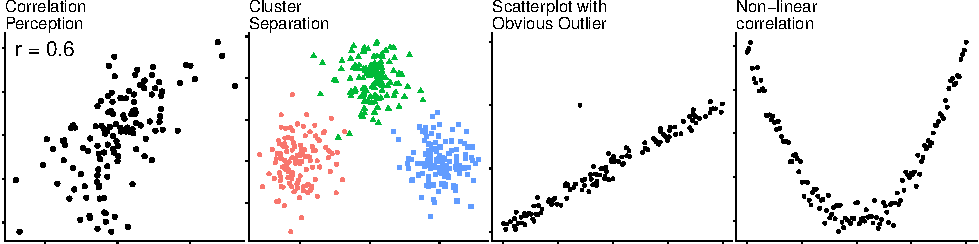
\includegraphics[width=1\textwidth,height=\textheight]{size_and_contrast_files/figure-pdf/fig-tasks-1.pdf}

}

\caption{\label{fig-tasks}Examples of scatterplots designed for
different scatterplot-associated tasks. Both color and point shape have
been used to delineate different clusters in the cluster separation
plot.}

\end{figure}

\hypertarget{sec-related-work}{%
\section{Related Work}\label{sec-related-work}}

\hypertarget{sec-testing-corr-percept}{%
\subsection{Testing Correlation
Perception}\label{sec-testing-corr-percept}}

The testing of linear correlation perception in scatterplots has a long
and rich history, and has explored a wide variety of plot types, tasks,
and modeling methods. Work has involved participants engaged in making
discrimination judgements between scatterplots with different
correlations \citep{pollack_1960, doherty_2007}, finding that
performance on such tasks became better as the objective \emph{r} value
increased. This performance on a discrimination judgement task can also
be modeled by deep neural networks \citep{yang_2023}. Extensive work
throughout the 1970s to 1990s focused primarily on having participants
produce a numerical estimate of correlation, and found evidence for a
systematic \emph{underestimation} for positive \emph{r} values besides 0
and 1. This underestimation was especially pronounced for 0.2
\textless{} \emph{r} \textless{} 0.6
\citep{strahan_1978, bobko_1979, cleveland_1982, lane_1985, lauer_1989, collyer_1990, meyer_1992}
and is demonstrated using an equation relating objective to subjective
correlation \citep{rensink_2017} in
Figure~\ref{fig-underestimation-curve}. More recent work has attempted
to model participants' correlation estimation performance by using a
combination of a bisection task, in which participants are asked to
adjust a plot until its correlation is halfway between that of two
reference plots, and a staircase method task designed to produce Just
Noticeable Differences between scatterplots such that they are
discriminable 75\% of the time \citep{rensink_2010}. This work has also
been extended to incorporate Bayesian data analysis \citep{kay_2015},
which is in agreement with other literature identifying scatterplots as
particularly suited for correlation perception \citep{li_2010}. The
current experiment adapts techniques from previous work
\citep{strain_2023, strain_2023b} and combines them to further push the
envelope of how systematically adjusting visual features in scatterplots
can radically alter people's perceptions of correlation. For this reason
we use the same direct estimation paradigm to collect responses. This
paradigm allows for a large number of judgements to be collected, and is
simple enough that participants need little to no training.

\hypertarget{sec-drivers}{%
\subsection{Drivers of Correlation Perception}\label{sec-drivers}}

Evidence points towards correlation perception being driven by the shape
of the underlying probability distribution represented by scatterplot
points, however it should be noted that this is very much still an open
question, especially with regards to what low level perceptual
mechanisms may be at play. It is possible that there are different
contributory perceptual mechanisms operating at different levels based
on task-specific differences such as viewing time or levels of
graph-training. Increasing the \emph{x} and \emph{y} scales on a
scatterplot such that the size of the point cloud decreases
\citep{cleveland_1982} is associated with an increase in a viewer's
judgements of bivariate association, despite the objective \emph{r}
value remaining the same. It was suggested in this case that viewers may
have been using the area of the point cloud to judge association. Later
work found that the relationship between objective and perceived
\emph{r} values could be described by a function that included the mean
of the geometric distances between the points and the regression line
\citep{meyer_1997}. Investigation of the idea that people use visual
features to judge correlation provides evidence that, among other
features, the standard deviation of all perpendicular distances from
scatterplot points to the regression line is predictive of performance
on a correlation estimation task \citep{yang_2019}. Equations for both
discrimination and magnitude estimation of \emph{r} in scatterplots
include a quantity that is small when \emph{r} = 1 and increases as
\emph{r} approaches 0 \citep{rensink_2017}. This quantity is indifferent
to the type of visualization used, and is functionally similar to that
found in work mentioned above
\citep{cleveland_1982, meyer_1997, yang_2019}. Regarding scatterplots,
this quantity represents the average distance between data points and
the regression line, and can be thought of as representing the width of
the underlying probability distribution. Findings from a convolutional
neural network that learnt visual features related to correlation
perception also support the idea that viewers are using an aspect of
scatterplot shape to judge correlation, or some measure of what has been
termed \emph{dot entropy} \citep{yang_2023}, again considered a
candidate visual proxy for correlation judgements
\citep{rensink_2017, rensink_2022}.

Recent work investigating the use of decay functions that change point
size or contrast in scatterplots as a function of residual distance
provide further evidence for both point density and salience/perceptual
weighting being drivers of correlation perception. The use of an
inverted contrast decay function \citep{strain_2023}, such that the
contrast of a point decreased the closer it was to the regression line,
resulted in significantly lower and less accurate correlation estimates
compared to uniformly full-contrast plots with the same overall shape.
This finding suggests that the lower contrast in the center of the
scatterplot biased viewers' perceptions down. When point contrast or
size are reduced as a function of distance from the regression line
\citep{strain_2023, strain_2023b}, viewers rate correlation as
significantly higher and are significantly more accurate. This supports
a low-level data salience account. Our aims are to test the impact of
systematically altering visual features on correlation perception and to
provide empirically-derived tools for visualization designers to design
better visualizations informed by the use of a simple, reproducible
framework.

\begin{figure}

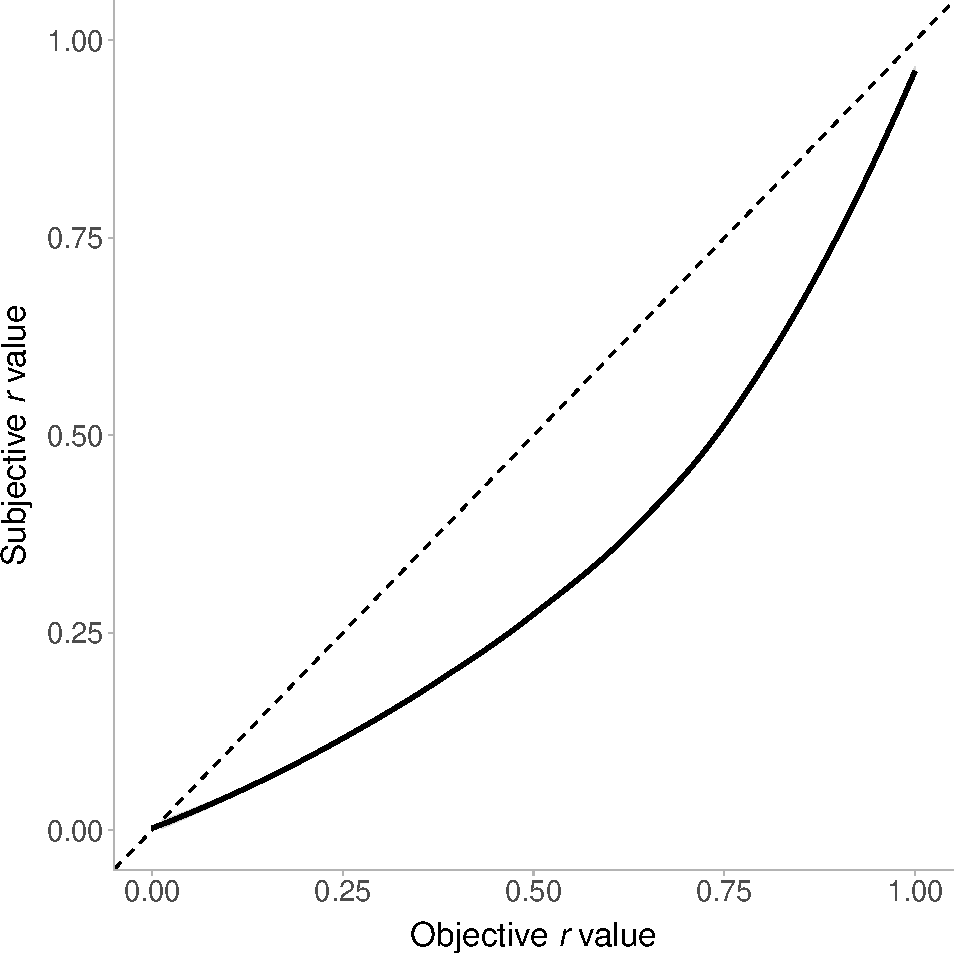
\includegraphics[width=0.5\textwidth,height=\textheight]{size_and_contrast_files/figure-pdf/fig-underestimation-curve-1.pdf} \hfill{}

\caption{\label{fig-underestimation-curve}Using a function relating
objective to perceived \emph{r} value \citep{rensink_2017} provides a
visualization of the nature of correlation underestimation reported in
previous work. An identity line has been included to illustrate where
viewers are most and least accurate.}

\end{figure}

\hypertarget{sec-transparency-and-contrast}{%
\subsection{Transparency and
Contrast}\label{sec-transparency-and-contrast}}

\begin{figure}

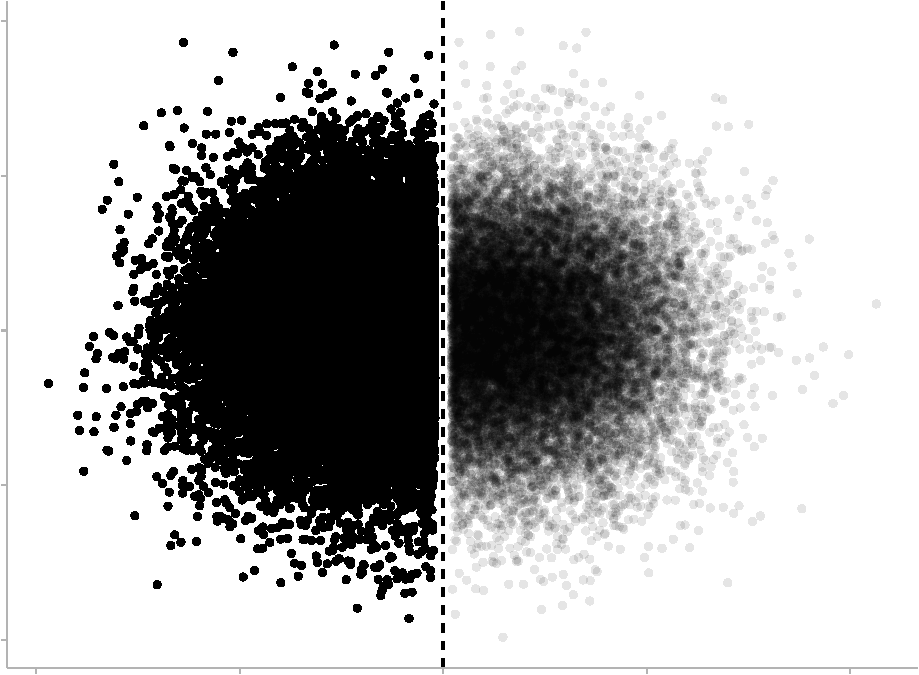
\includegraphics[width=0.5\textwidth,height=\textheight]{size_and_contrast_files/figure-pdf/fig-overplotting-examples-1.pdf} \hfill{}

\caption{\label{fig-overplotting-examples}Adjusting point contrast to
address overplotting. Contrast between the points and the background is
full (alpha = 1, L) or low (alpha = .1, R). The dataset used has 40,000
points.}

\end{figure}

\begin{figure}

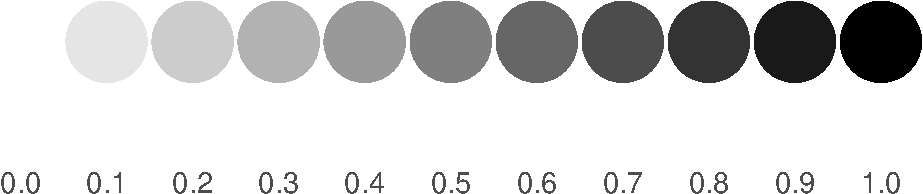
\includegraphics[width=0.5\textwidth,height=\textheight]{size_and_contrast_files/figure-pdf/fig-alpha-examples-1.pdf} \hfill{}

\caption{\label{fig-alpha-examples}Demonstrating the effects of
different alpha values on point contrast.}

\end{figure}

Changing the contrast of scatterplot points is standard practice to deal
with issues of overplotting \citep{matejka_2015, bertini_2004};
scatterplots with very large numbers of points, especially with high
degrees of overlap, suffer from low individual-point visibility caused
by high point density. Lowering the contrast of all points addresses
this, and makes data trends and distributions easier to see and
interpret (see Figure~\ref{fig-overplotting-examples}). In the present
study we use the \textbf{ggplot2} package \citep{hadley_gg2016} to
create our stimuli. This package uses an alpha parameter, or the level
of linear interpolation \citep{stone_2008} between foreground and
background pixel values, to set the contrast of points. As demonstrated
in Figure~\ref{fig-alpha-examples}, an alpha value of 0 or 1 results in
no interpolation and rendering of either the background or foreground
pixel values respectively. Psychophysical definitions of perceived
contrast are often based on what is being presented (e.g., gratings) or
are modeled to take into account aspects of human vision (e.g.,
visibility limits) \citep{zuffi_2007}. Our crowdsourced methodology
gives us no control over the exact luminances of our stimuli, only over
the \emph{relative} differences in luminance between scatterplot points
and backgrounds. For this reason we do not report absolute luminance nor
make any attempt to adopt a formal definition of contrast; instead we
report the alpha value used. Given that our work aims to improve
correlation perception without removing data from the scatterplot, we
also incorporate point visibility testing (see Section~\ref{sec-VT}).
Informal point visibility piloting suggested that our smallest, lowest
contrast points had very low visibility. We therefore implemented an
alpha = 0.2 floor for these points, which we judged as conferring a
sufficient level of point visibility.

Previous work has found that lowering the contrast of \emph{all}
scatterplot points relative to the background can increase the level of
underestimation error relative to full contrast, and that lowering point
contrast \emph{as a function of distance from the regression line} is
able to bias correlation estimates upwards to partially correct for the
underestimation observed \citep{strain_2023}. Evidence suggests point
salience/perceptual weighting or spatial uncertainty as drivers for this
effect. Lower stimulus contrast is associated with lower salience
\citep{healey_2011}, can bias judgements of mean point position
\citep{hong_2021}, increase error in positional judgements
\citep{wehrhahn_1990}, and can result in greater uncertainty in speed
perception \citep{champion_2017}. Due to mechanistic accounts of both
salience/perceptual weighting and spatial uncertainty predicting results
in the same direction, previous work \citep{strain_2023} has been unable
to determine the extent to which each is responsible for the observed
reduction in correlation estimation error.

\hypertarget{sec-point-size}{%
\subsection{Point Size}\label{sec-point-size}}

For discriminability reasons, scatterplots visualizing large datasets
tend also to have smaller points. Bubble charts are a subclass of
scatterplot which use point size to describe a third variable, but what
little experimental work there is on the impact of point size on
correlation perception is inconclusive. Some work has found bias and
variability in correlation perception to be invariant to changes in
point size \citep{rensink_2012, rensink_2014}, while elsewhere a strong
effect of changing point size as a function of distance from the
regression line has been reported \citep{strain_2023b}. Evidence points
towards a salience-dominant mechanism in the latter case, albeit with a
small effect of spatial uncertainty. There is evidence that larger
stimulus size is associated with lower levels of spatial certainty
\citep{alais_2004}, but higher levels of salience \citep{healey_2011}.
The predicted effects of these drivers on correlation perception work in
the opposite direction to one another, which has allowed researchers to
provide evidence for the mechanistic dominance of salience when point
size is used. When an inverted size decay function is used such that
smaller points are located nearer the regression line, correlation
estimation is significantly more accurate than when all points are the
same size \citep{strain_2023b}. In this case it was suggested that the
higher spatial uncertainty brought on by larger exterior points caused a
perceptual downweighting during correlation estimation, which is in line
with work suggesting our perceptual systems make robust use of
visuo-spatial information
\citep{strain_2023b, warren_2002, warren_2004}. This effect was small,
meaning we do not take it into account when making our hypotheses.

\hypertarget{hypotheses}{%
\subsection{Hypotheses}\label{hypotheses}}

We present a single experiment based on established effects of adjusting
point size and point contrast. In our study, we combine previously
independently tested point size and point contrast decay functions in
both standard orientation (contrast/size is reduced with residual
magnitude) and inverted orientation (contrast/size is increased with
residual magnitude). Throughout we refer to \emph{congruent} and
\emph{incongruent} conditions with respect to the orientations of size
and contrast decay functions. We hypothesize that: (H1) an increased
reduction in correlation estimation error will be observed when standard
orientation decay functions are used; (H2) the use of congruent inverted
orientation decay functions will produce the least accurate estimates of
correlation; and (H3) that owing to the greater strength of the size
channel observed in previous work \citep{strain_2023b}, there will be a
significant difference in correlation estimates between the two
incongruent orientation conditions.

\hypertarget{sec-methods}{%
\section{Methodology}\label{sec-methods}}

\hypertarget{sec-crowdsourcing}{%
\subsection{Crowdsourcing}\label{sec-crowdsourcing}}

Much prior work into correlation perception in scatterplots has taken
place in-person, most often with graduate students with experience in
statistics. While this work is valuable, especially to perception
audiences, it can struggle to provide data that is resilient to
different viewing contexts and the wide range of levels of statistical
and graph experience present in lay populations. In addition, the ease
and low-cost afforded to us by online, crowdsourced experimental work is
unmatched. Given our intended HCI and design audience, we therefore
choose to crowdsource all participants. We acknowledge however, that the
technique has been affected by low quality data and skewed demographics
in the past \citep{chmielewski_2020, charalambides_2021, peer_2021}. In
light of these issues we follow published guidelines \citep{peer_2021}
to ensure the collection of high quality data. Namely, we use the
Prolific.co platform \citep{prolific} with stringent pre-screen
restrictions; participants were required to have completed at least 100
studies using Prolific, and were required to have a prolific score of
100, representing a 99\% approval rate. This is more strict than the
95\% suggested in previous work \citep{peer_2021}, but has served the
authors well in prior work.

\hypertarget{sec-open-research}{%
\subsection{Open Research}\label{sec-open-research}}

This study was conducted according to the principles of open and
reproducible research \citep{ayris_2018}. All data and analysis code are
available at (repository link removed for anon). This repository
contains instructions for building a Docker container to fully reproduce
the computational environment used. This allows for full replications of
stimuli, analysis, and the paper itself. Ethical approval was granted by
(removed for anon). Hypotheses and analysis plans were pre-registered
with the OSF (links removed for anon) and there were no deviations from
them.

\hypertarget{sec-scatter-gen}{%
\subsection{Stimuli}\label{sec-scatter-gen}}

45 scatterplot datasets were generated corresponding to 45 \emph{r}
values uniformly distributed between 0.2 and 0.99, as there is evidence
that very little correlation is perceived below \emph{r} = 0.2
\citep{strahan_1978, bobko_1979, cleveland_1982}. Using so many values
for \emph{r} allows us to paint a broader picture of people's perception
than work using fewer values. Scatterplot points were generated based on
bivariate normal distributions with standard deviations of 1 in each
direction. Each scatterplot had a 1:1 aspect ratio, was generated as a
1000 x 1000 pixel .png image, and was scaled up or down according to a
participant's monitor such that they always occupied the same proportion
of the screen. We used equation 1 to map residuals to size and contrast
values. When adjusting point size, we further transform values using a
scaling factor of 4 and a constant of 0.2 to ensure that the minimum
point size in the present study is both visible and consistent with that
of previous work \citep{strain_2023, strain_2023b}.

\begin{equation}
  point_{size/contrast} = 1 - b^{residual}
\end{equation}

0.25 was chosen as the value of \emph{b}. This value was used in
previous studies that the present work builds upon, and it produces a
curve approximating the inverse around the identity line of the
underestimation curve reported in previous work
\citep{rensink_2017, strain_2023, strain_2023b}. We acknowledge that
there may be other, more suitable values of \emph{b}, however extensive
testing of these is outside the scope of the present work. We used this
equation in standard and inverted orientation forms applied to point
size and contrast in a factorial 2 x 2 design. Examples of the stimuli
used can be seen in Figure~\ref{fig-examples}.

\begin{figure}

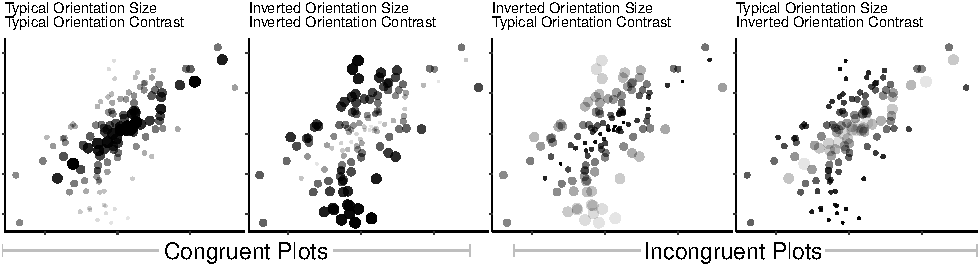
\includegraphics[width=0.5\textwidth,height=\textheight]{size_and_contrast_files/figure-pdf/fig-examples-1.pdf} \hfill{}

\caption{\label{fig-examples}Examples of the experimental stimuli used.
Congruent conditions are at the top, while incongruent conditions are
below.}

\end{figure}

\hypertarget{sec-gen-modelling}{%
\subsection{Modeling}\label{sec-gen-modelling}}

We use linear mixed effects models to model the relationships between
the combination of size and contrast decay functions and participants'
errors in correlation estimates. Models such as these allow us to
compare differences in our IV across the full range of participant
responses, as opposed to relying purely on aggregate data, as in ANOVA.
These models also afford us the ability to include random effects for
participants and items. As per our pre-registrations we preferred
maximal models, including random intercepts and slopes for participants
and items. The structures of these models were identified using the
\textbf{buildmer} package in R (version 2.10.1,
\citep{voeten_buildmer}). This package takes a maximal random effects
structure and then identifies the most complex model that converges by
dropping terms that fail to explain a significant amount of variance.

\hypertarget{sec-VT}{%
\subsection{Point Visibility Testing}\label{sec-VT}}

Discussions about the size and contrast of particular scatterplot points
are inherently difficult in the context of online, crowdsourced
experiments; controlling the devices participants use to participate in
these kinds of experiments, beyond insisting on laptop or desktop
computers, is impossible. While this may result in a lack of consistency
in scatterplot point sizes, luminances, or contrast ratios between
participants, it also provides results that are more resilient to
different viewing contexts than traditional lab-based experimental work.
In addition to measures implemented to ensure high quality participant
data (see Section~\ref{sec-crowdsourcing}), it is also key that we do
not inadvertently remove data from scatterplots by including points
whose size or contrast renders them invisible. We therefore included
point visibility testing to check this. Participants viewed six
scatterplots that were made up of a certain number of points between 2
and 7. These points were of the same size and contrast as the smallest
and lowest contrast points used in the experimental items. Participants
were asked to enter in a textbox how many points were present.
Participants scored an average of 74.89\% (\(SD\) = 32.25\%). Despite
our use of the contrast floor detailed in
Section~\ref{sec-transparency-and-contrast}, it is clear that some of
our small, low contrast points were not reliably visible, most likely
due to low contrast between the point and background, as previous work
\citep{strain_2023b} found point visibility largely invariant to size.
We suggest this is due to differences in monitor specifications between
participants. In reality minimum visible size and contrast would need to
be calibrated on a per-monitor basis. We also include performance on the
point visibility test as a fixed effect in
Section~\ref{sec-add-analyses}.

\hypertarget{sec-dot-pitch}{%
\subsection{Dot Pitch}\label{sec-dot-pitch}}

We employed a method for obtaining the dot pitch of participants'
monitors \citep{screenscale}. Combining this with monitor resolution
information allows us to calculate the physical on-screen size of
scatterplot points. Participants were asked to hold a standard size
credit/debit/ID card (ISO/IEC 7810 ID-1) up to their screen and resize
an on-screen card until their sizes matched. We assumed a widescreen
16:9 aspect ratio and calculated dot pitch based on these measurements.
Mean dot pitch was 0.34mm (\(SD\) = 0.05), corresponding to a physical
onscreen size of 4.39mm on a 1920 x 1080 pixel monitor for the smallest
points displayed. We include analyses with dot pitch as a fixed effect
in Section~\ref{sec-add-analyses}.

\hypertarget{sec-gen-procedure}{%
\subsection{Procedure}\label{sec-gen-procedure}}

Both experiments were built using PsychoPy \citep{pierce_2019} and
hosted on Pavlovia.org. Participants were only permitted to complete the
experiment on a desktop or laptop computer. Each participant was first
shown the participant information sheet and provided consent through key
presses in response to consent statements. They were asked to provide
their age in a free text box, followed by their gender identity.
Participants completed the 5-item Subjective Graph Literacy test
\citep{garcia_2016}, followed by the point visibility task described in
Section~\ref{sec-VT} and the screen scale task described in
Section~\ref{sec-dot-pitch}. Participants were given instructions, and
were then shown examples of scatterplots with correlations of \emph{r} =
0.2, 0.5, 0.8, and 0.95, as piloting of a previous experiment indicated
some of the lay population may be unfamiliar with the visual character
of scatterplots. Section~\ref{sec-add-analyses} contains further
analysis of the potential training effects of this. Two practice trials
were given before the experiment began. Participants worked through a
randomly presented series of 180 experimental trials and were asked to
use a slider to estimate correlation to 2 decimal places. Visual masks
preceded each scatterplot. Interspersed were 6 attention check trials
which explicitly asked participants to ignore the scatterplot and set
the slider to 0 or 1.

\hypertarget{sec-participants}{%
\subsection{Participants}\label{sec-participants}}

150 participants were recruited using the Prolific.co platform. Normal
to corrected-to-normal vision and English fluency were required for
participation. In addition, participants who had completed any of our
previous studies into correlation estimation in scatterplots (references
removed for anon) were prevented from participating. Data were collected
from 158 participants. 8 failed more than 2 out of 6 attention check
questions, and, as per pre-registration stipulations, were rejected from
the study. Data from the remaining 150 participants were included in the
full analysis (50.7\% male, 48.7\% female, and 0.7\% non-binary).
Participants' mean age was 30.6 (\emph{SD} = 8.6). Participants' mean
graph literacy score was 22.5 (\emph{SD} = 3.5). The average time taken
to complete the experiment was 37 minutes (\emph{SD} = 12.3).

\hypertarget{sec-design}{%
\subsection{Design}\label{sec-design}}

We used a fully repeated-measures 2 x 2 factorial design. Each
participant saw each combination of size and contrast decay function
plots for a total of 180 experimental items. Participants viewed these
experimental items, along with 6 attention check items, in a fully
randomized order. All experimental code, materials, and instructions are
hosted at (link removed for anon).

\hypertarget{sec-results}{%
\section{Results}\label{sec-results}}

Our first two hypotheses were fully supported in this experiment. The
combination of standard orientation size and contrast decay functions
produced the most accurate estimates of correlation, although this also
resulted in a large over-correction and consequent overestimation for
many values of \emph{r} (see Figure~\ref{fig-diff-error-bars-plot}). Our
second hypothesis was also supported; the combination of inverted size
and inverted contrast decay functions produced the least accurate
estimates of correlation. We found no support for our third hypothesis;
there was no significant difference in correlation estimates between
standard orientation size/inverted orientation contrast decay plots and
inverted orientation size/standard orientation contrast decay plots (Z =
-2.26, \emph{p} = .11), however we did find a significant interaction
effect that provides evidence that the combination of size and contrast
decay functions is not additive in nature.

\hypertarget{tbl-sig}{}
\begin{table}
\caption{\label{tbl-sig}Significances of fixed effects and the interaction between them.
Semi-partial R\textsuperscript{2} for each fixed effect and the
interaction term is also displayed in lieu of effect sizes. }\tabularnewline

\centering
\begin{tabular}{lrrrrll}
\toprule
  & Estimate & Standard Error & df & t-value & \textit{p} & R\textsuperscript{2}\\
\midrule
(Intercept) & 0.08 & 0.013 & 103.32 & 6.27 & <0.001 & \\
Size Decay & -0.14 & 0.005 & 148.39 & -25.77 & <0.001 & 0.104\\
Contrast Decay & 0.12 & 0.002 & 26327.21 & 63.71 & <0.001 & 0.087\\
Size Decay x Contrast Decay & 0.15 & 0.004 & 26327.13 & 38.47 & <0.001 & 0.034\\
\bottomrule
\end{tabular}
\end{table}

All analyses were conducted using R (version 4.3.1). Deviation coding
was used for each of the experimental factors. We used the
\textbf{buildmer} and \textbf{lme4} (version 1.1-34 \citep{lme4})
packages to build a linear mixed effects model where the difference
between objective and rated \emph{r} value was predicted by the size and
contrast decay functions used. A likelihood ratio test revealed that the
model including point size and contrast decay conditions as fixed
effects explained significantly more variance than the null
(\(\chi^2\)(3) = 5,286.81, \emph{p} \textless{} .001). There were
significant fixed effects of size decay and contrast decay, as well as a
significant interaction between the two. The experimental model has
random intercepts for items and participants, and a random slope for the
size decay factor with regards to participants. Due both to our use of a
linear mixed model with an interaction term, and our lack of a
comparative baseline condition (i.e no size or contrast function used),
we do not report a measure of effect size. Instead we report the amounts
of variance explained by each fixed effect term and the interaction term
as semi-partial R\textsuperscript{2} \citep{nakagawa_2013}. These values
were calculated using the \textbf{r2glmm} package (version 0.1.2
\citep{r2glmm}) and can be see in Table~\ref{tbl-sig} along with all
model statistics. The \textbf{emmeans} package (version 1.8.8
\citep{emmeans}) was used to calculate pairwise comparisons between
levels of the size and contrast decay factor, and can be seen in
Table~\ref{tbl-contrasts}.

\begin{figure}

{\centering 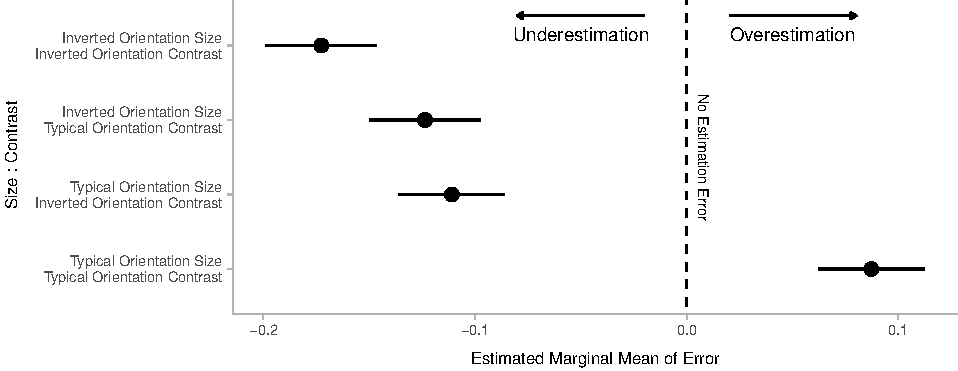
\includegraphics[width=1\textwidth,height=\textheight]{size_and_contrast_files/figure-pdf/fig-emm-plot-1.pdf}

}

\caption{\label{fig-emm-plot}Estimated marginal means for each
combination of size and contrast decay conditions, including asymptotic
lower and upper confidence intervals.}

\end{figure}

\hypertarget{tbl-contrasts}{}
\begin{table}
\caption{\label{tbl-contrasts}Pairwise comparisons. SO = Standard Orientation, IO = Inverted
Orientation. The interaction is driven by the non-additive nature of
combining point size and contrast decay functions, and the only
nonsignificant contrast is found when incongruent decay functions are
compared. }\tabularnewline

\centering
\begin{tabular}{lrl}
\toprule
Contrast & Z.ratio & \textit{p}\\
\midrule
SO Size x IO Contrast <-> IO Size x IO Contrast & -10.95 & <0.001\\
SO Size x IO Contrast <-> SO Size x SO Contrast & 72.29 & <0.001\\
SO Size x IO Contrast <-> IO Size x SO Contrast & -2.26 & 0.108\\
IO Size x IO Contrast <-> SO Size x SO Contrast & 46.13 & <0.001\\
IO Size x IO Contrast <-> IO Size x SO Contrast & 17.84 & <0.001\\
\addlinespace
SO Size x SO Contrast <-> IO Size x SO Contrast & -37.44 & <0.001\\
\bottomrule
\end{tabular}
\end{table}

\begin{figure}

{\centering 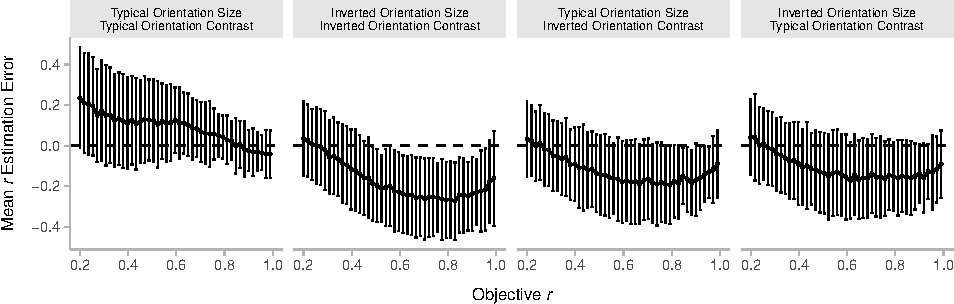
\includegraphics[width=1\textwidth,height=\textheight]{size_and_contrast_files/figure-pdf/fig-diff-error-bars-plot-1.pdf}

}

\caption{\label{fig-diff-error-bars-plot}Plots showing how participants'
correlation estimation errors change as a function of the \emph{r} value
for each combination of size and contrast decay factors. Overestimation
occurs above the dashed line.}

\end{figure}

\hypertarget{sec-add-analyses}{%
\subsection{Additional Analyses}\label{sec-add-analyses}}

We find no effects of graph literacy (\(\chi^2\)(1) = 3.50, \emph{p} =
.061), performance on the point visibility task (\(\chi^2\)(1) = 1.29,
\emph{p} = .257), or dot pitch (\(\chi^2\)(1) = 1.52, \emph{p} = .218)
on participants' errors in correlation estimation. We did find a
significant effect of training (\(\chi^2\)(1) = 23.78, \emph{p}
\textless{} .001), with participants rating correlation .01 lower during
the second half. While this effect is statistically significant, we do
not consider it large enough to warrant further discussion.

\hypertarget{sec-discussion}{%
\section{Discussion}\label{sec-discussion}}

The finding of a significant interaction between point size and contrast
decay provides evidence that these functions interact in non-additive
ways. In addition, we provide further confirmatory evidence of what has
been found previously. Namely, that while manipulations of both point
size and contrast have significant effects, the effect of changing point
size is stronger, and that while we can influence correlation estimates
in either direction, standard orientation manipulations are more
powerful than inverted ones \citep{strain_2023, strain_2023b}. As one
would expect, we also see an effect of orientation congruency on the
extent to which a manipulation can bias correlation estimates. The lack
of support for our third hypothesis, that there would be a difference in
correlation estimates between incongruent conditions, was surprising
given the greater strength of the size channel relative to contrast
demonstrated in previous work \citep{strain_2023, strain_2023b},
although this may be a facet of the non-additive interaction between
size and contrast manipulations we found. Despite the lack of support
for this hypothesis, we did find that the size decay channel explained
more variance (.104) in our model than contrast decay (.087) was able
to.

Taking into account the present work, which manipulates point size and
contrast together, and previous work manipulating the same visual
features in isolation, we provide recommendations to visualization
designers and researchers:

\begin{itemize}
\tightlist
\item
  The size decay function in isolation should be used when \emph{r} is
  between approximately 0.3 and 0.75. In this range it produces the most
  accurate \emph{r} estimates in participants.
\item
  Outside of this range, the contrast decay function should be used in
  isolation, as here it produces the most accurate \emph{r} estimates.
\item
  There exists a combination of size and contrast decay functions that
  produces accurate correlation estimates while maintaining the
  increased \emph{r} estimation precision that we would expect to see
  with high \emph{r} values. Finding this will require extensive future
  testing.
\end{itemize}

\hypertarget{sec-combining}{%
\subsection{Combining Manipulations}\label{sec-combining}}

Figure~\ref{fig-emm-plot} and Figure~\ref{fig-diff-error-bars-plot} show
how, on average, the combination of standard orientation size and
contrast decay functions has resulted in an overestimation of \emph{r}
for the majority of values. While this does not directly solve the
underestimation problem, it does demonstrate that with regards to using
point size and contrast to bias viewer's estimates of correlation in
scatterplots, there would appear to be few limitations. If we can
over-correct correlation estimates, then we certainly have the ability
to correct appropriately. The issue here is not one of our
\emph{ability} to change people's perceptions, but of \emph{tuning} the
use of these visual factors to be able to change people's perceptions in
systematic ways. We explore what further work would need to be done to
do this in Section~\ref{sec-future-work}. Combining inverted size and
contrast decay functions also had the predicted effect in this case,
producing the lowest and least accurate estimates of correlation.
Combining inverted manipulations did not, however, significantly change
the shape of the estimation curve (see
Figure~\ref{fig-diff-error-bars-plot}). In addition to interacting
non-additively, the effects we observe operate differently depending on
the direction of the change induced in perception. This finding can also
explain the lack of support found for our hypothesis that there would be
a significant difference in \emph{r} estimation error between the two
incongruent conditions. Despite the size channel being more powerful
with regards to influencing correlation estimates, the fact that this
power depends on the direction the function is set causes incongruent
functions to act against each other in ways we would not expect. Indeed,
the incongruent condition that used a standard orientation size decay
function did exhibit lower mean error than the one using inverted size
decay (see Figure~\ref{fig-diff-error-bars-plot}), however in each case
the contrast decay appears to have blunted the power of the size decay
function to the extent that the difference in errors is not
statistically significant.

\hypertarget{estimation-precision}{%
\subsection{Estimation Precision}\label{estimation-precision}}

Much previous work is consistent with regards to the finding that
\emph{r} estimation precision increases with the objective \emph{r}
value
\citep{rensink_2010, rensink_2012, rensink_2014, rensink_2017, doherty_2007}.
More recent work using size or contrast decay functions similar to the
ones used here \citep{strain_2023, strain_2023b} has found that in some
cases, precision in \emph{r} estimation is \emph{constant} across the
range of \emph{r} values investigated. For example, the use of a size
decay function, whether using standard/inverted orientation non-linear
functions or a linear decay function, results in \textbf{no} change in
\emph{r} estimation precision \citep{strain_2023b}. When contrast is
used in the same ways, only an inverted decay function \textbf{does not}
exhibit the conventional increase in precision with \emph{r}. In the
present work, precision in \emph{r} estimation increased whenever a
standard orientation contrast decay function was used. We suggest this
is part of the moderating effect of the point contrast decay function on
the size decay function; the visual character of scatterplots with high
\emph{r} values that use the size decay function eliminates the usual
increase in precision we would expect, however the introduction of the
contrast decay function normalizes this to the point where precision is
restored.

\hypertarget{contributions-of-size-and-contrast-decay}{%
\subsection{Contributions of Size and Contrast
Decay}\label{contributions-of-size-and-contrast-decay}}

Incorporating data from previous work \citep{strain_2023, strain_2023b}
that used similar decay functions and experimental paradigms allows us
to compare estimation curves for size decay and contrast decay in
isolation and in combination. Figure~\ref{fig-est-multi-exp} shows
correlation estimation error curves in the present experiment and in two
previous studies that used decay functions applied solely to size or
contrast.

\begin{figure}

{\centering 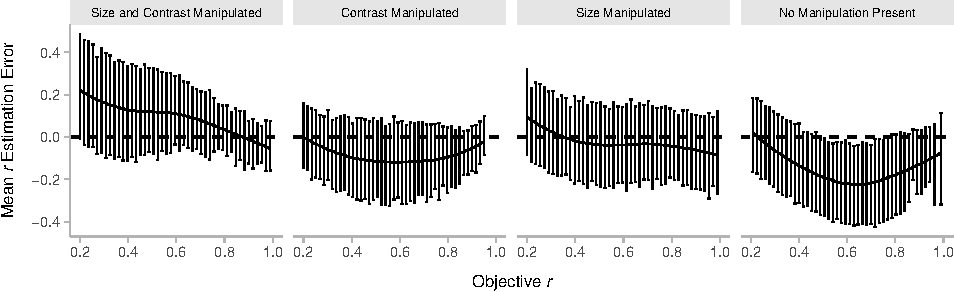
\includegraphics[width=1\textwidth,height=\textheight]{size_and_contrast_files/figure-pdf/fig-est-multi-exp-1.pdf}

}

\caption{\label{fig-est-multi-exp}Plotting \emph{r} estimation error
against the objective \emph{r} value for contrast and size decay in
isolation from previous work, and for their combination in the present
study. The dashed line represents 0 error in correlation estimation, and
standard deviations are shown as error bars. Note that these curves have
been smoothed. Overestimation occurs above the dashed line. The plot
line for the plot without manipulation was averaged from previous work.}

\end{figure}

Using contrast decay alone does not significantly change the shape of
the estimation error curve, whereas using size decay does. When size and
contrast decay functions are combined, however, the shape appears
similar to that of size alone. This is in line with previous work
establishing size as a more potent channel for the manipulation of
correlation estimates \citep{strain_2023b}. It would appear that the
addition of the contrast curve moderates the effect of the size curve as
a function of the objective \emph{r} value itself, without affecting the
general shape of the curve. In the following, we briefly discuss the
effects of each manipulation in isolation and the manipulations
together, before making a case for the inclusion of both when tuning
scatterplots for correlation estimation due to the complementary
benefits each confers. Throughout the course of this section it should
be noted that the analyses include data from several separate
experiments. We argue that their methodological similarities render
comparison appropriate, but we acknowledge the potential for overstated
conclusions.

Using a contrast decay function in isolation has a small effect on
correlation estimation. It does little to change the shape of the
underestimation curve (see Figure~\ref{fig-underestimation-curve}), but
slightly biases \emph{r} estimates up to partially correct for the
underestimation observed with standard scatterplots \citep{strain_2023}.
Importantly, it also preserves the increase in correlation estimation
precision that we would expect to find during correlation estimation
tasks. Using the size decay function in isolation has a more dramatic
effect. The shape of the estimation curve is altered quite radically,
and there is no increase in precision with the objective \emph{r} value
\citep{strain_2023b}. Size decay over-corrects at lower values of
\emph{r}, leading to an overestimation effect, while at high values the
curve begins to change direction, leading to a more severe
underestimation. In the middle range of \emph{r} values, however, the
size decay function in isolation performs well. One option for tuning
correlation estimation using these functions would therefore be to use
the size decay function in isolation for mid-range values of \emph{r}
(0.3 to 0.75), and to use the contrast decay function in isolation
outside of this range. Used together however, we can exploit the power
of the size decay function whilst maintaining the expected increase in
precision with \emph{r} that the contrast decay function confers. It is
clear that the simple combination we have used in the present study does
not represent an ideal tuning, as participants overestimated \emph{r}
for the majority of values, but this confirms that there is the scope to
bias \emph{r} estimates significantly using the functions supplied here.
Further work would be required to obtain precise measures of the power
of each decay function and their power together. Doing this would allow
us to tune each function according to both objective \emph{r} value and
the tuning of the other function to produce accurate correlation
estimates. We can derive new curves that describe the effect that each
manipulation and the combination of manipulations has on correlation
estimates (Figure~\ref{fig-power-plot}) by comparing them to estimates
without any manipulation present. We term this `power'. The dotted line
on each plot shows the power we would need to correct for the standard
underestimation curve (see Figure~\ref{fig-underestimation-curve}). As
we can see, size alone provides the closest to the requirement, and
combining size and contrast decay functions results in gross
overestimation.

\begin{figure}

{\centering 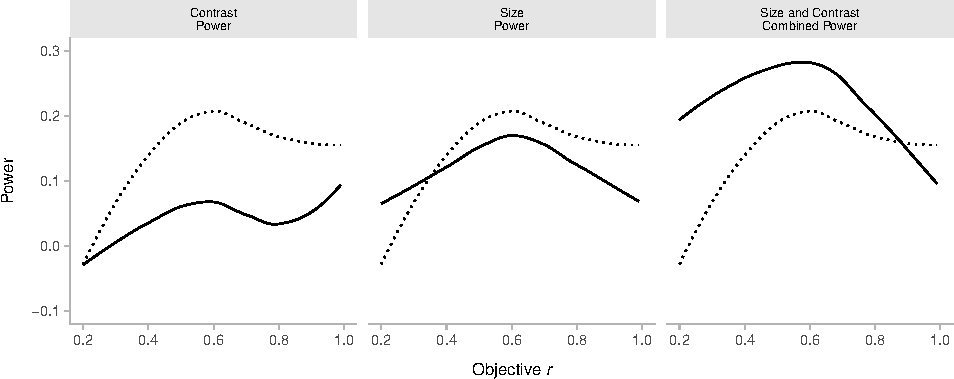
\includegraphics[width=1\textwidth,height=\textheight]{size_and_contrast_files/figure-pdf/fig-power-plot-1.pdf}

}

\caption{\label{fig-power-plot}Power is the difference between what is
observed when a decay function/combination of decay functions is used
and what is observed when no manipulation is used. The dashed line
represents the power that would be required to correct for the observed
underestimation of correlation in scatterplots.}

\end{figure}

\hypertarget{sec-mechs}{%
\subsection{Mechanisms}\label{sec-mechs}}

Previous work has made the case for contrast and size decay acting
primarily through salience/perceptual weighting, with the caveat that
spatial certainty also plays a small part in the mechanism behind size
decay \citep{strain_2023, strain_2023b}. Our results are supportive of
this notion, with our lowest and highest estimates being observed in the
incongruent and congruent conditions respectively. These findings also
support dot density \citep{yang_2023} and feature-based attentional bias
accounts \citep{hong_2021, sun_2016}. As all of these mechanisms would
be expected to operate in the same direction, making conclusions about
the relative contributions of each is difficult. The body of evidence
generally points to a high-level probability distribution account
\citep{rensink_2017, rensink_2022}. On a lower level, numerous candidate
mechanisms exist, which are mostly expected to act in the same
direction. Previous work concluded that spatial certainty
\citep{strain_2023b} may play a small role with regards to the effects
of size decay on correlation perception; our results neither confirm nor
refute this, but instead provide further evidence for
salience/perceptual weighting/dot density changing participants'
perceptions of the width of a probability distribution to affect
correlation estimates.

\hypertarget{sec-limitations}{%
\subsection{Limitations}\label{sec-limitations}}

Firstly, our participants' performance on the point visibility task was
poor, with an average score of only 74.89\%. It is clear from these
results that for many participants, the smallest and lowest contrast
points we used were simply not visible, although it would seem that this
low visibility had no significant effect on correlation estimates.
Regardless, for many of our participants it will have appeared that we
were removing data, which goes against our intended aims. Solving this
would require a by-participant calibration of point size and point
contrast, which is beyond the scope of our current methodology, as it
would require stimuli to be fully re-generated for each participant. We
aim to implement this in the future, although it would require a
different platform, such as a server-based instance of Rstudio being run
in the background to re-generate stimuli per a calibration task
completed by the participant. We cannot say precisely what proportions
of the observed effect in the standard orientation congruent condition
were due to size or contrast decay. We can conclude that these effects
are not linearly additive, but must suggest further work to define
precisely each of their contributions.

\hypertarget{sec-future-work}{%
\subsection{Future Work}\label{sec-future-work}}

There is evidence that viewers overestimate correlation in negatively
correlated scatterplots \citep{sher_2017}. Future work may make use of
the functions and findings we have provided to begin solving this
problem. We found evidence that the influence of size and contrast decay
functions changes according to the direction they are operating in,
meaning experimental work with negatively correlated scatterplots would
be required, and results may differ significantly from findings related
to the underestimation of correlation in positively correlated
scatterplots. For size and contrast decay in the present work we used
equation 1. Given our finding that the combination is non-additive,
there are a multitude of adjustable parameters for each decay function
that require rigorous testing in order to produce concrete values of the
contributions of each. The value of \emph{b} is one such parameter. We
used the same value of \emph{b} (0.25) as in previous work
\citep{strain_2023, strain_2023b}. Changing this value can increase or
decrease the severity of the effect in question. Additionally, we used a
constant and a scaling factor with the size decay manipulation to ensure
our points were visible. These values could also be changed. Aside from
changing aspects of equation 1, there are other equations that could be
used, including ones that take into account objective \emph{r} value to
change the values used to set point size or contrast. The present work
opens the door for this future work, as it provides the necessary
additional data to previous experiments using only size
\citep{strain_2023b} or contrast \citep{strain_2023} decay functions.
Further testing of these manipulations in isolation and combination
using different decay function parameters will allow researchers to
build a more complete picture of how these visual features impact
correlation estimation, and how we can exploit them to correct for a
historic bias.

Through this work we also provide an example of an experimental
framework that we argue should be employed to test a wider range of data
visualizations, statistical summaries, and task types. Our framework is
fully open source, and can be easily adapted for other charts and
modalities. Doing this furthers the cause of empirically-informed data
visualization design.

\bibliographystyle{ACM-Reference-Format}
\bibliography{size-contrast.bib}

%% begin pandoc before-bib
%% end pandoc before-bib
%% begin pandoc biblio
%% end pandoc biblio
%% begin pandoc include-after
%% end pandoc include-after
%% begin pandoc after-body
%% end pandoc after-body

\end{document}
\endinput
%%
%% End of file `sample-manuscript.tex'.
